\documentclass[1,DS,p,e,prof]{phBook}
%\documentclass[../coursseconde]{subfiles}
%Options : 2, 1, T, SNT (classes), p, b,prof, exos, cours, DS, noir, a4, a5, twocolumn, landscape
\def\datedevoir{6/01/26} % date du DS à indiquer

\graphicspath{{figures/}}

\begin{document}
\setcounter{chapter}{3} %Numéro du chapitre précédent
\chapter{\prof{CORRECTION}\eleve{NOM : \hfill Devoir
}} %Titre du chapitre
%%%%%%%%%%%%%%%%%%%%%%%%



    % sens de variations des fonctions : deux quadratiques, trois fonctions du troisième degré de sorte que pour f'(x) soient avec  \Delta de signes différents, une fraction rationnelle, une de la forme ax+b/x.
    \begin{enonce}
        Pour chacune des fonctions suivantes :
        \begin{itemize}
            \item Calculer la dérivée \(f'(x)\).
            % \item Étudier le signe de \(f'(x)\).
            \item Déterminer les sens de variations de la fonction \(f\).
        \end{itemize}
        \begin{enumerate}
            \item \(f(x)=x^2-4x+3\).
            \item \(f(x)=-2x^2+4x+5\).
            \item \(f(x)=-x^3+3x^2-3x+2\).
            % \item \(f(x)=x^3-6x^2+9x+1\).
            \item \(f(x)=-2x^3+3x^2+12x-5\).
            \item \(f(x)=\dfrac{2x+1}{x-2}\) définie sur \(\mathbb{R}\setminus\{2\}\).
            \item \(f(x)=3x+\dfrac{48}{x}\), définie sur \(\mathbb{R}\setminus\{0\}\).
        \end{enumerate}
    \end{enonce}
    \begin{correction} % assistée par IA
        \begin{enumerate}
            \item \(f(x)=x^2-4x+3\).
            
            La dérivée d'une fonction polynôme s'obtient en dérivant terme par terme :
            \[f'(x) = 2x - 4\]
            % Calcul vérifié
            
            Étudions le signe de \(f'(x)\) :
            \begin{align*}
            f'(x) &= 0 \\
            2x - 4 &= 0 \\
            x &= 2
            \end{align*}
            
            Le coefficient de \(x\) dans \(f'(x)\) est positif (2), donc \(f'(x)\) est négative avant 2 et positive après 2.
            
            \begin{center}
              \begin{tikzpicture}[scale=0.7]
              \tkzTabInit[lgt=2,espcl=2]{$x$/1, $f'(x)$/1, $f(x)$/2}{$-\infty$, $2$, $+\infty$}
              \tkzTabLine{, -, z, +, }
              \tkzTabVar{+/, -/$-1$, +/}
              \end{tikzpicture}
            \end{center}
            
            La fonction \(f\) est décroissante sur \(]-\infty;2]\) et croissante sur \([2;+\infty[\).
            
            \item \(f(x)=-2x^2+4x+5\).
            
            \[f'(x) = -4x + 4\]
            % Calcul vérifié
            
            Étudions le signe de \(f'(x)\) :
            \begin{align*}
            f'(x) &= 0 \\
            -4x + 4 &= 0 \\
            x &= 1
            \end{align*}
            
            Le coefficient de \(x\) dans \(f'(x)\) est négatif (-4), donc \(f'(x)\) est positive avant 1 et négative après 1.
            
            \begin{center}
              \begin{tikzpicture}[scale=0.7]
              \tkzTabInit[lgt=2,espcl=2]{$x$/1, $f'(x)$/1, $f(x)$/2}{$-\infty$, $1$, $+\infty$}
              \tkzTabLine{, +, z, -, }
              \tkzTabVar{-/, +/$7$, -/}
              \end{tikzpicture}
            \end{center}
            
            La fonction \(f\) est croissante sur \(]-\infty;1]\) et décroissante sur \([1;+\infty[\).
            
            \item \(f(x)=-x^3+3x^2-3x+2\).
            
            \[f'(x) = -3x^2 + 6x - 3 = -3(x^2 - 2x + 1) = -3(x-1)^2\]
            % Calcul vérifié
            
            La dérivée \(f'(x) = -3(x-1)^2\) est toujours négative ou nulle (elle s'annule en \(x=1\)).
            
            \begin{center}
              \begin{tikzpicture}[scale=0.7]
              \tkzTabInit[lgt=2,espcl=2]{$x$/1, $f'(x)$/1, $f(x)$/2}{$-\infty$, $1$, $+\infty$}
              \tkzTabLine{, -, z, -, }
              \tkzTabVar{+/, -/$1$, -/}
              \end{tikzpicture}
            \end{center}
            
            La fonction \(f\) est strictement décroissante sur \(\mathbb{R}\).
            
            \item \(f(x)=-2x^3+3x^2+12x-5\).
            
            \[f'(x) = -6x^2 + 6x + 12 = -6(x^2 - x - 2)\]
            % Calcul vérifié
            
            Résolvons \(f'(x) = 0\) :
            \(x^2 - x - 2 = 0\)
            
            Calculons \(\Delta\) :
            \[\Delta = b^2 - 4ac = (-1)^2 - 4(1)(-2) = 1 + 8 = 9\]
            % Calcul vérifié
            
            Les racines sont :
            \[x_1 = \frac{1-3}{2} = -1 \quad \text{et} \quad x_2 = \frac{1+3}{2} = 2\]
            % Calcul vérifié
            
            Le coefficient de \(x^2\) dans \(f'(x)\) est négatif (-6), donc \(f'(x)\) est négative à l'extérieur des racines et positive entre les racines.
            
            \begin{center}
              \begin{tikzpicture}[scale=0.7]
              \tkzTabInit[lgt=2,espcl=2]{$x$/1, $f'(x)$/1, $f(x)$/2}{$-\infty$, $-1$, $2$, $+\infty$}
              \tkzTabLine{, -, z, +, z, -, }
              \tkzTabVar{+/, -/$-12$, +/$15$, -/}
              \end{tikzpicture}
            \end{center}
            
            La fonction \(f\) est décroissante sur \(]-\infty;-1]\), croissante sur \([-1;2]\) et décroissante sur \([2;+\infty[\).
            
            \item \(f(x)=\dfrac{2x+1}{x-2}\) définie sur \(\mathbb{R}\setminus\{2\}\).
            
            Utilisons la formule de dérivation d'un quotient : \(\left(\frac{u}{v}\right)' = \frac{u'v - uv'}{v^2}\)
            
            Avec \(u = 2x+1\) et \(v = x-2\), on a \(u' = 2\) et \(v' = 1\).
            
            \[f'(x) = \frac{2(x-2) - (2x+1)(1)}{(x-2)^2} = \frac{2x-4-2x-1}{(x-2)^2} = \frac{-5}{(x-2)^2}\]
            % Calcul vérifié
            
            Comme \((x-2)^2 > 0\) pour tout \(x \neq 2\), on a \(f'(x) < 0\) sur tout le domaine de définition.
            
            \begin{center}
              \begin{tikzpicture}[scale=0.7]
              \tkzTabInit[lgt=2,espcl=2]{$x$/1, $f'(x)$/1, $f(x)$/2}{$-\infty$, $2$, $+\infty$}
              \tkzTabLine{, -, d, -, }
              \tkzTabVar{+/, -/d, -/}
              \end{tikzpicture}
            \end{center}
            
            La fonction \(f\) est strictement décroissante sur \(]-\infty;2[\) et sur \(]2;+\infty[\).
            
            \item \(f(x)=3x+\dfrac{48}{x}\), définie sur \(\mathbb{R}\setminus\{0\}\).
            
            On peut écrire \(f(x) = 3x + 48x^{-1}\), donc :
            \[f'(x) = 3 + 48 \times (-1) \times x^{-2} = 3 - \frac{48}{x^2}\]
            % Calcul vérifié
            
            Étudions le signe de \(f'(x)\) :
            \begin{align*}
            f'(x) &= 0 \\
            3 - \frac{48}{x^2} &= 0 \\
            3 &= \frac{48}{x^2} \\
            3x^2 &= 48 \\
            x^2 &= 16 \\
            x &= \pm 4
            \end{align*}
            % Calcul vérifié
            
            Pour déterminer le signe de \(f'(x) = 3 - \frac{48}{x^2} = \frac{3x^2 - 48}{x^2}\), étudions le signe du numérateur \(3x^2 - 48 = 3(x^2-16) = 3(x-4)(x+4)\).
            
            \begin{center}
              \begin{tikzpicture}[scale=0.7]
              \tkzTabInit[lgt=2,espcl=2]{$x$/1, $f'(x)$/1, $f(x)$/2}{$-\infty$, $-4$, $0$, $4$, $+\infty$}
              \tkzTabLine{, +, z, -, d, -, z, +, }
              \tkzTabVar{-/, +/$-24$, -/d, -/$24$, +/}
              \end{tikzpicture}
            \end{center}
            
            La fonction \(f\) est croissante sur \(]-\infty;-4]\), décroissante sur \([-4;0[\) et sur \(]0;4]\), et croissante sur \([4;+\infty[\).
        \end{enumerate}
    \end{correction}

%%%%%%%%%%%%%%%%%
% Fin exercice %%
%%%%%%%%%%%%%%%%%



\begin{exercice}
    \begin{enonce}
        Donner les variations de $f(x)=\frac{2x-1}{x+3}$ sur son domaine de définition.
    \end{enonce}
    %%%%%%%%%%%

    \begin{correction}
        
    \end{correction}
\end{exercice}
%%%%%%%%%%%%%%%%%%%%%
%%% Fin exercice %%%%
%%%%%%%%%%%%%%%%%%%%%








\end{document}
